\section{Product}
\subsection{Current Status of Product}
In the current state, the driving capabilities of WTR have been improved considerably.
The functionality of WTR has been improved through inclusion of an IMU, rotary encoders and the sonar sensors.
While some of these were present at the start of the project, data was either being spoofed or simply not being utilized.

The IMU previously used, the MPU6050, for example was not actually used, and the data was being spoofed so that the robot would move more smoothly.
This has now been corrected, and the actual data received from the new MPU9250 is incorporated into the planning, as well as being more accurate than the old IMU.

The sonars, which previously were not used, are now utilized as well.
Several additional sensors are now located at the back of WTR, so that it can also detect obstacles behind it.
This means that even during reversing the likelihood of a collision is massively reduced.

\subsection{What Could Be Added?}
There are some features that could be implemented in order to increase the safety features of WTR, which are all documented in the separate section security [\ref{sec::security}].

\subsection{Schematic Overview}
Figure [\ref{fig::schemView}] shows the new situation of WTR.
More detailed explanations of every section can be found in the respective documents dealing with those sections, such as the hardware and tech designs.
\begin{figure}[H]
\centering
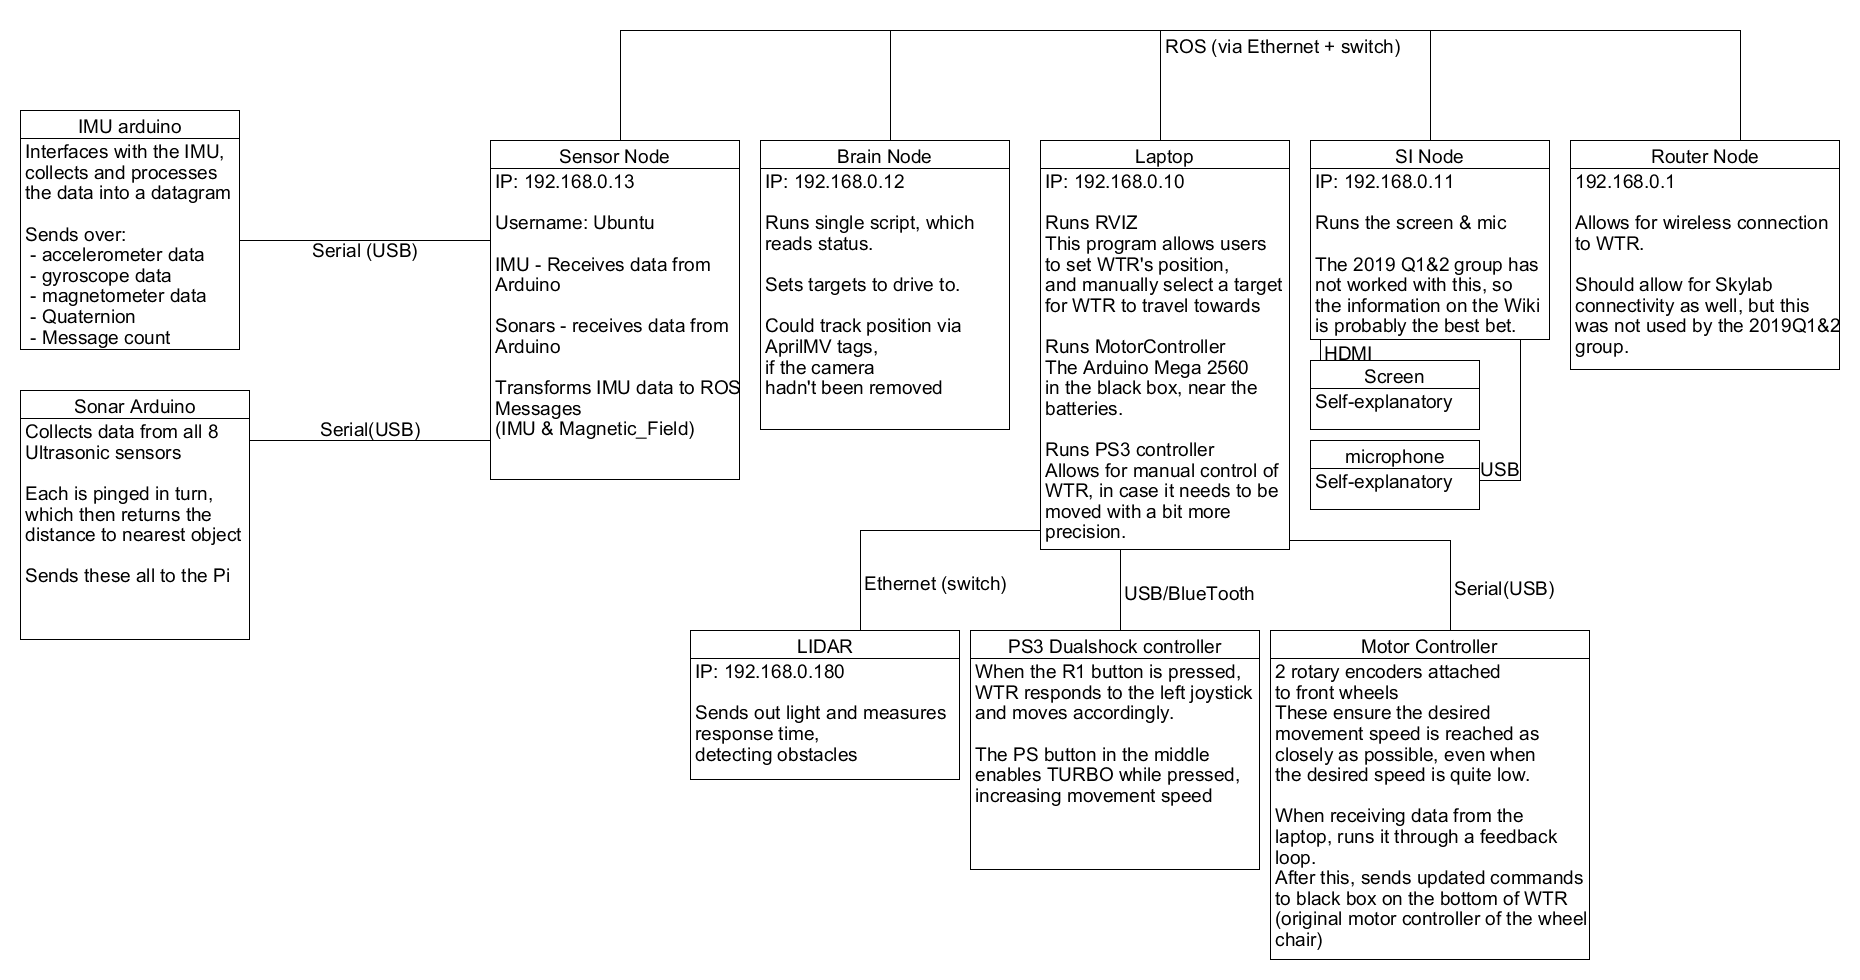
\includegraphics[width=15cm]{rosOverview.png}
\caption{An overview of the separate parts of WTR}
\label{fig::schemView}
\end{figure}

The sensor node communicates with the IMU and the sonar HC-SR04 sensors through arduinos over a serial communication protocol.
This allows for updates or maintenance to either component without having to shut down the entire robot, as WTR can still function without these, albeit at a reduced accuracy of autonomous movement.
This allows features to be tested separately from WTR before adding them to the complete robot.

The motor controller is an Arduino Mega 2560, which is connected to the laptop through a USB cable and uses a serial communication protocol as well to translate the commands from RVIZ to a format the P\&G [\ref{trm::PGE}] can understand and execute.
The feedback loop ensures that it can perform accurately at low velocity as well, rather than blindly sending a speed to it and assuming it is accurate enough to do so.

\newpage
